\documentclass{beamer}
\usetheme{default}
\beamertemplatenavigationsymbolsempty
\usepackage{rembeamer}

\begin{document}

\begin{frame}
  \begin{itemize}
    \item[] 
      Using the normal distribution to conduct hypothesis tests for a
      difference in proportions and interpreting the results. 
  \end{itemize}
\end{frame}

\begin{frame}
  \frametitle{Difference in Proportions}
  \begin{itemize}
    \item[] 
      Two categorical variables: one dependent and one explanatory. 
      \vspace{0.5cm}
    \item[] 
      Each with two categories: two input groups in the explanatory
      variable, two outcomes in the dependent variable. 
      \vspace{0.5cm}
    \item[] 
      Perfect for controled trials: does a malaria vaccine reduce the
      rate of infection with malaria?
  \end{itemize}
\end{frame}

\begin{frame}
  \frametitle{An Psychology Example}
  \begin{itemize}
    \item[] 
      Question: do you want to buy a DVD for a discounted price of
      \$15? 
      \vspace{0.5cm}
    \item[] 
      \begin{smallitemize}
        \item
          Buy the DVD.
        \item
          Don't buy the DVD.
      \end{smallitemize}
      \vspace{0.5cm}
    \item[] 
      \begin{smallitemize}
        \item
          Buy the DVD.
        \item
          Don't buy the DVD, and keep the \$15 for other purchases.
      \end{smallitemize}
      \vspace{0.5cm}
    \item[] 
      150 subjects, 75 in each group. 
  \end{itemize}
\end{frame}

\begin{frame}
  \frametitle{Contingency Table}
  \begin{table}
    \begin{tabular}{@{}cccc@{}}
      \toprule
      Group & Buy & Do Not Buy & Total \\
      \cmidrule(r){1-1} \cmidrule(rl){2-2} \cmidrule(rl){3-3}
      \cmidrule(l){4-4}
      Control & 56 & 19 & 75 \\[0.3em]
      Treatment & 41 & 34 & 75 \\[0.3em]
      Total & 97 & 53 & 150 \\
      \bottomrule
    \end{tabular}
  \end{table}
\end{frame}

\begin{frame}
  \frametitle{Standardized Bar Plot}
  \centering
  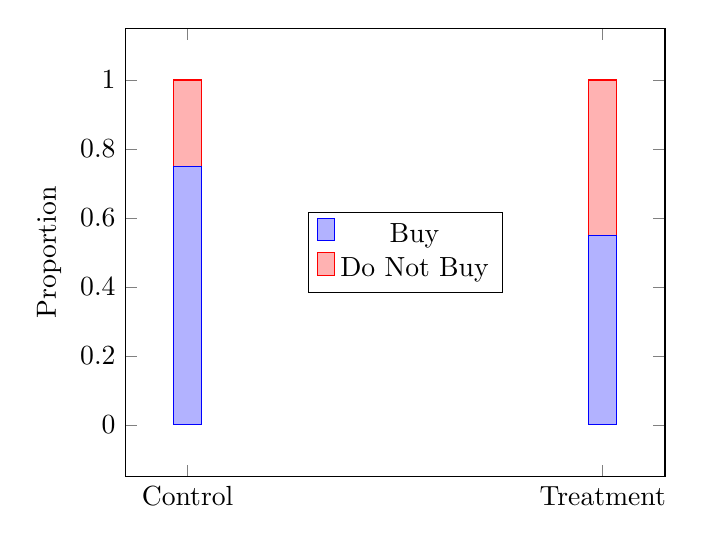
\begin{tikzpicture}
    \begin{axis}[
      ybar stacked,
      ymin=0,
      enlargelimits=0.15,
      legend style={at={(0.70,0.5)}, anchor=east},
      ylabel={Proportion},
      symbolic x coords={Control,Treatment},
      xtick=data,
    ]
    \addplot+ [ybar] coordinates {(Control,0.75) (Treatment,0.55)};
    \addplot+ [ybar] coordinates {(Control,0.25) (Treatment,0.45)};
    \legend{Buy,Do Not Buy}
  \end{axis}
  \end{tikzpicture}
\end{frame}

\begin{frame}
  \frametitle{Statistics and Hypotheses}
  \begin{displaymath}
    \begin{array}{rcl}
      \hat{p}_T - \hat{p}_C & = & \frac{34}{75} - \frac{19}{75} =
      0.453 - 0.253 = 0.200 \\[2em]
      H_0:\quad p_T - p_C & = & 0 \\[2em]
      H_A:\quad p_T - p_C & > & 0
    \end{array}
  \end{displaymath} 
\end{frame}

\begin{frame}
  \frametitle{Simulation}
  \centering
  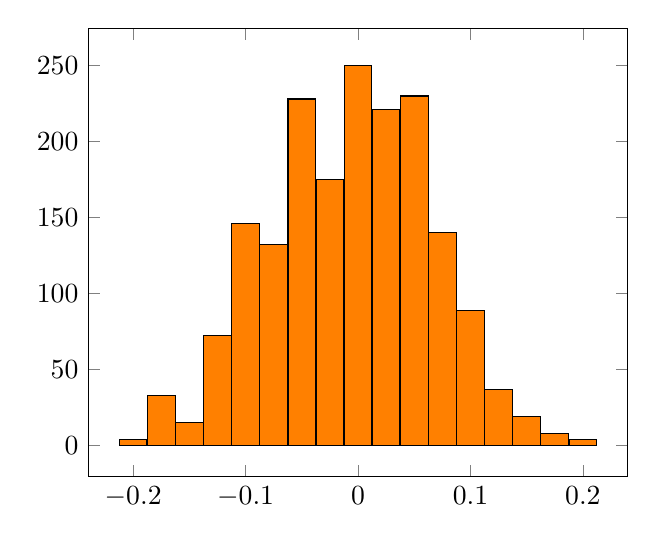
\begin{tikzpicture}
    \begin{axis}
    \addplot [
      ybar,
      ylabel={Count},
      fill=orange,
    ] coordinates {
    (-0.2,4)
    (-0.175,33)
    (-0.15,15)
    (-0.125,72)
    (-0.1,146)
    (-0.075,132)
    (-0.05,228)
    (-0.025,175)
    (0,250)
    (0.025,221)
    (0.05,230)
    (0.075,140)
    (0.1,89)
    (0.125,37)
    (0.15,19)
    (0.175,8)
    (0.2,4)
    };
  \end{axis}
  \end{tikzpicture}
  \begin{equation*}
    p = 0.6%
  \end{equation*}
\end{frame}

\begin{frame}
  \frametitle{Normal Distribution}
  \centering
  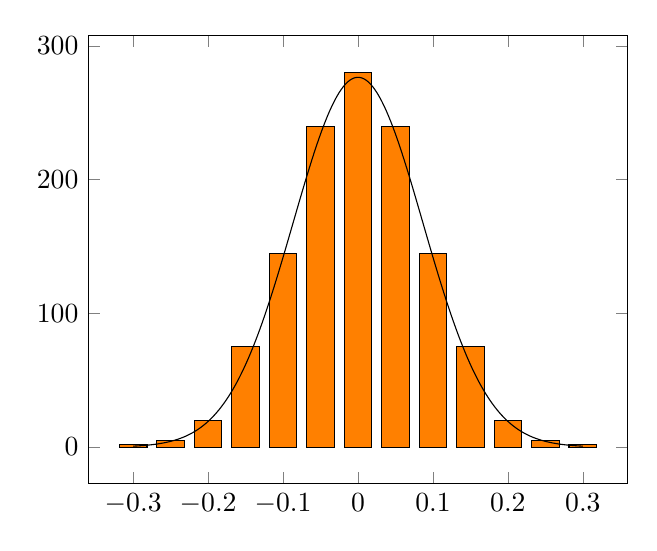
\begin{tikzpicture}
    \begin{axis}
    \addplot [
      ybar,
      ylabel={Count},
      fill=orange,
    ] coordinates {
    (-0.3,2)
    (-0.25,5)
    (-0.2,20)
    (-0.15,75)
    (-0.1,145)
    (-0.05,240)
    (0,280)
    (0.05,240)
    (0.1,145)
    (0.15,75)
    (0.2,20)
    (0.25,5)
    (0.3,2)
    };
    \addplot [
      domain=-0.3:0.3,
      samples=200,
    ]
    {60*exp(-x^2 / 0.015) / sqrt(2*pi*0.0075))};
  \end{axis}
  \end{tikzpicture}
\end{frame}

\begin{frame}
  \frametitle{Z-Scores}
  \begin{displaymath}
    \begin{array}{rcl}
      z(x) & = & \frac{x - \mu}{\sigma} \\[2em]
      z & = & \frac{0.2 - 0}{0.078} = 2.56\\[2em]
      \text{Percentile} & = & 0.9948 \\[2em]
      p & = & 1 - 0.9948 = 0.0052 \\[2em]
      p & < & 0.05
    \end{array}
  \end{displaymath} 
\end{frame}

\begin{frame}
  \frametitle{Standard Deviation for a Sampling Distribution for a Difference of Proportions} 
  \begin{displaymath}
    \begin{array}{rcl}
      \text{Difference in Proportions} & & p_1 - p_2 \\[2em]
      \text{Category 1 Sample Size} & = & n_1 \\[2em]
      \text{Category 2 Sample size} & = & n_2 \\[2em]
      \sigma & = & \sqrt{\frac{p_1(1-p_1)}{n_1} +
      \frac{p_2(1-p_2)}{n_2}}\\[2em]
      \sigma & \mapsto & SE 
    \end{array}
  \end{displaymath} 
\end{frame}

\begin{frame}
  \frametitle{Calculating Standard Error}
  \begin{equation*}
    \sigma = \sqrt{\frac{p_1(1-p_1)}{n_1} + \frac{p_2(1-p_2)}{n_2}}
  \end{equation*}
  \begin{table}
    \begin{tabular}{@{}cccc@{}}
      \toprule
      Group & Buy & Do Not Buy & Total \\
      \cmidrule(r){1-1} \cmidrule(rl){2-2} \cmidrule(rl){3-3}
      \cmidrule(l){4-4}
      Control & 56 & 19 & $n_1 = 75$ \\[0.3em]
      Treatment & 41 & 34 & $n_2 = 75$ \\[0.3em]
      Total & 97 & 53 & 150 \\
      \bottomrule
    \end{tabular}
  \end{table}
\end{frame}

\begin{frame}
  \frametitle{Calculating Standard Error}
  \begin{equation*}
    \sigma = \sqrt{\frac{p_1(1-p_1)}{n_1} + \frac{p_2(1-p_2)}{n_2}}
  \end{equation*}
  \begin{table}
    \begin{tabular}{@{}cccc@{}}
      \toprule
      Group & Buy & Do Not Buy & Total \\
      \cmidrule(r){1-1} \cmidrule(rl){2-2} \cmidrule(rl){3-3}
      \cmidrule(l){4-4}
      Control & 56 & 19 & $n_1 = 75$ \\[0.3em]
      Treatment & 41 & 34 & $n_2 = 75$ \\[0.3em]
      Total & 97 & 53 & 150 \\
      \bottomrule
    \end{tabular}
  \end{table}
  \begin{equation*}
    p_1 = p_2 = \frac{53}{150} = 0.35 
  \end{equation*}
\end{frame}

\begin{frame}
  \frametitle{Calculating Standard Error} 
  \begin{displaymath}
    \begin{array}{rcl}
      \sigma & = & \sqrt{\frac{p_1(1-p_1)}{n_1} +
      \frac{p_2(1-p_2)}{n_2}} \\[2em]
      & = & \sqrt{\frac{0.35(1-0.35)}{75} + \frac{0.35(1-0.35)}{75}}
      \\[2em]
      & = & 0.078
    \end{array}
  \end{displaymath} 
\end{frame}

\begin{frame}
  \frametitle{Hypothesis Testing for Difference in Proportions}
  \begin{itemize}
    \item[] 
      Calculate the sample statistic $x$. 
      \vspace{0.5cm}
    \item[] 
      Calculate the pooled proportion $p_{pool}$. 
      \vspace{0.5cm}
    \item[] 
      Calculate the standard error under the assumption of the null
      hypothesis.
      \vspace{0.5cm}
    \item[] 
      Calculate the z-score of the sample statistic.
      \vspace{0.5cm}
    \item[] 
      Use a table to get a percentile from the z-score.
      \vspace{0.5cm}
    \item[] 
      Subtract the percentile from 1 to get the p-value.
  \end{itemize}
\end{frame}

\end{document}

